%% This is an example first chapter.  You should put chapter/appendix that you
%% write into a separate file, and add a line \include{yourfilename} to
%% main.tex, where `yourfilename.tex' is the name of the chapter/appendix file.
%% You can process specific files by typing their names in at the 
%% \files=
%% prompt when you run the file main.tex through LaTeX.
\chapter{A novel analysis method for paired-sample microbial ecology experiments}

The contents of this chapter were published as: 
Olesen SW, Vora S, Techtmann SM, Fortney JL, Bastidas-Oyanedel JR, Rodr\'{i}guez J,
\textit{et al.} (2016) A Novel Analysis Method for Paired-Sample Microbial Ecology
Experiments. \textit{PLoS ONE} \textbf{11}(5): e0154804. doi:10.1371/journal.pone.0154804.

The figures, tables, and supplementary figures and tables are at the end of the chapter.

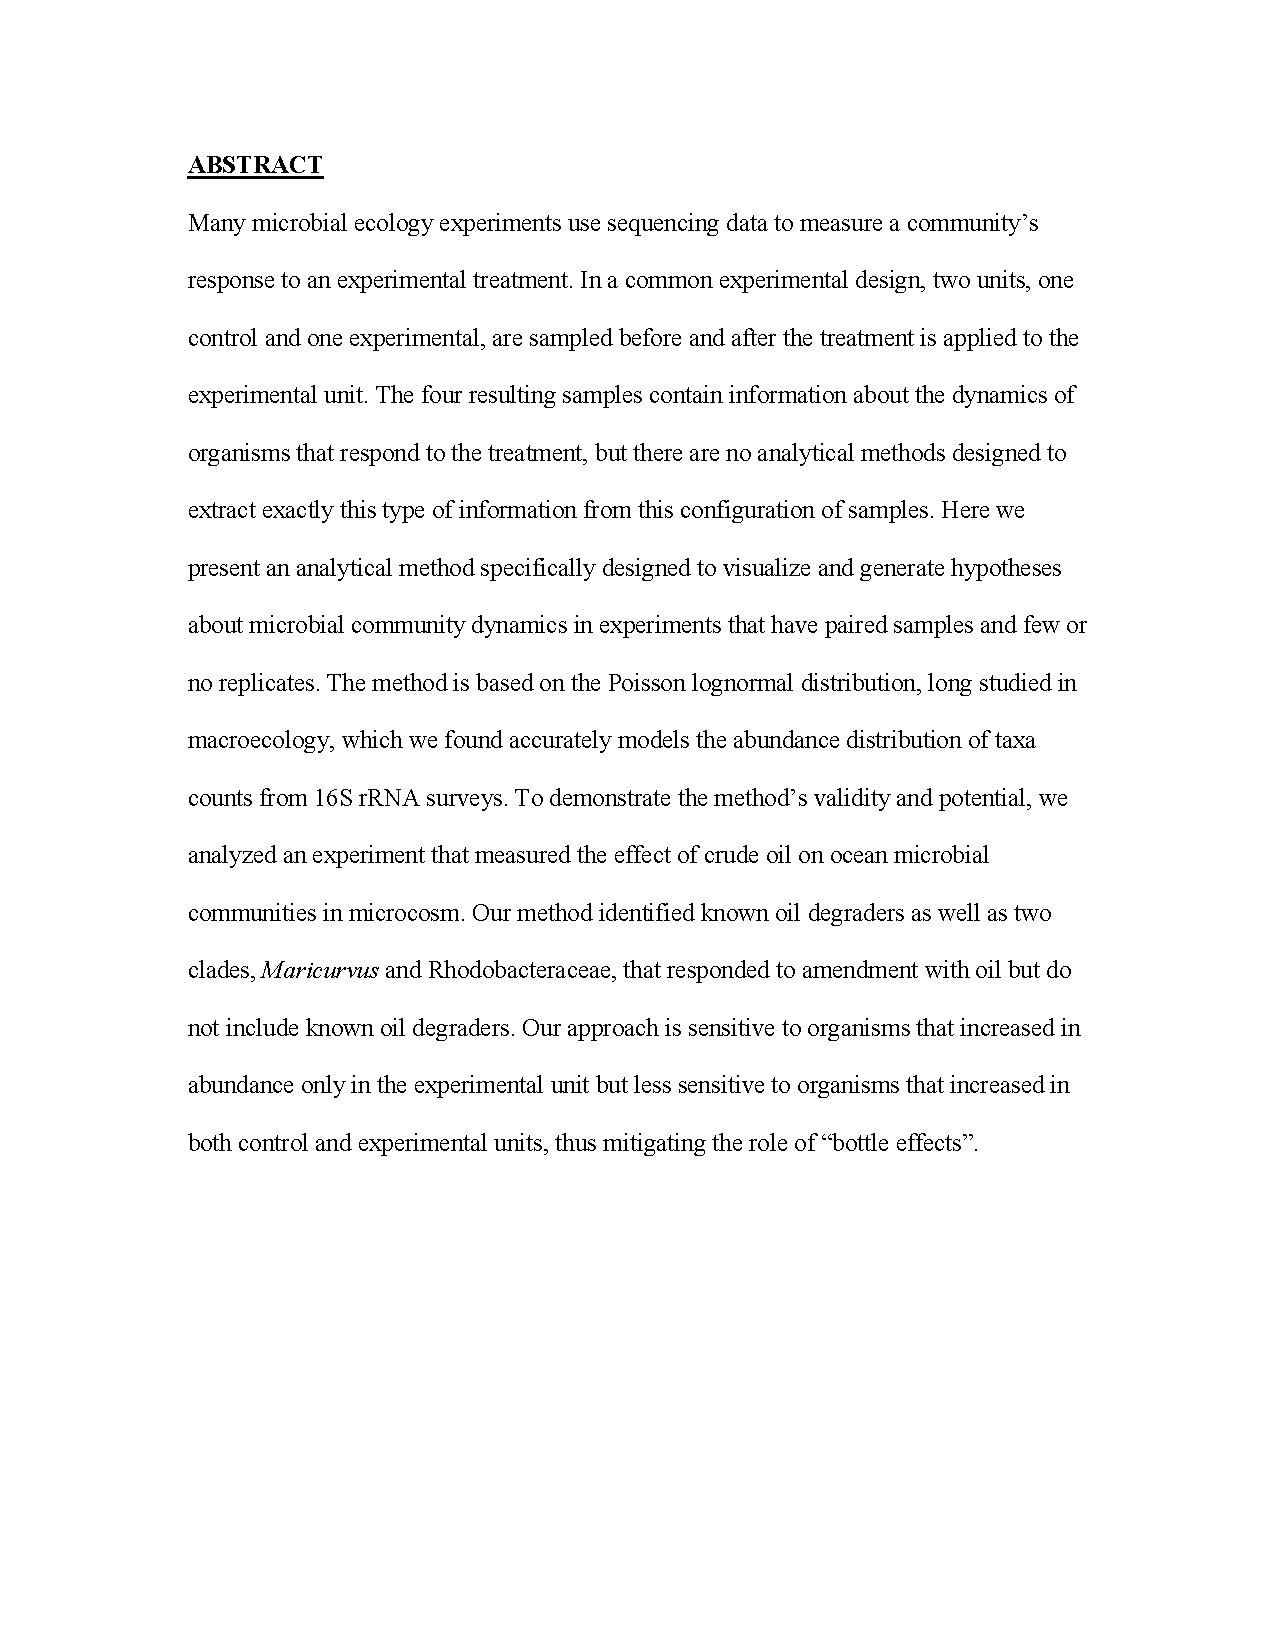
\includepdf[pages=-, pagecommand={\thispagestyle{plain}}, scale=1.0]{texmex/ms}

\clearpage
\begin{figure}[ht]
\centering
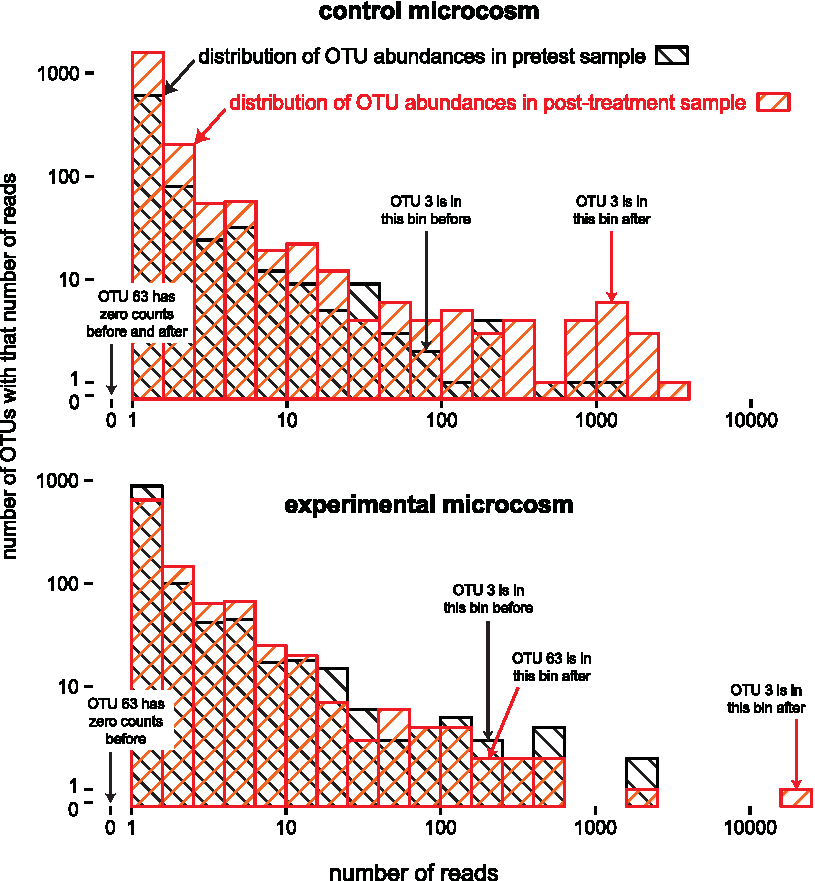
\includegraphics{texmex/fig/fig_1}
\caption*{{\bf Figure 1. OTU dynamics and possible bottle effects in a paired-sample experiment.} 
Four histograms are shown, one each for each sample in the experiment:
control-before (above, black), control-after (above, red), experimental-before
(below, black), experimental-after (below, red). Each histogram shows how many
OTUs (logarithmic $y$-axes) have what number of associated reads (logarithmic
$x$-axis). No bin is shown for OTUs with zero counts. The dynamics of two OTUs
are shown: black arrows point to the abundance bin for OTUs in the ``before''
sample and red arrows point their abundance bins in the ``after'' samples.}
\end{figure}

\clearpage
\begin{figure}[ht]
\centering
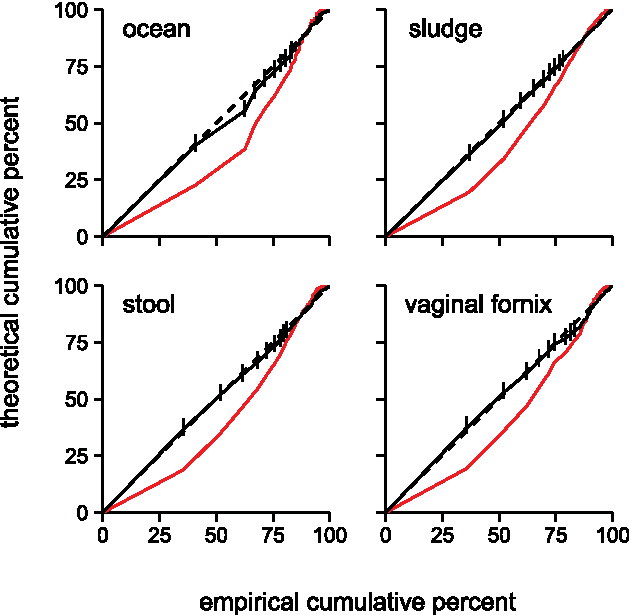
\includegraphics{texmex/fig/fig_2}
\caption*{{\bf Figure 2. TPL distribution fits OTU abundance distributions in multiple ecosystems.}
Probability-probability plots comparing the empirical cumulative distribution
function (horizontal axis) with the theoretical cumulative probability of a TPL
distribution fit to each data set (vertical axis, black solid line). The first
ten data points are marked with vertical dashes: the first dash (furthest lower
left) represents the fraction of OTUs that have 1 read, the second dash
represents the fraction of OTUs with 2 or fewer reads, and so forth. The dotted
black line indicates a perfect fit of the TPL to the empirical distribution ($y = x$).
The theoretical cumulative probability of a simple lognormal distribution
(red line) is shown to emphasize the quality of the TPL fit. The ecosystems are
ocean water from this study (top left), wastewater sludge from this study (top
right), human stool (bottom left; Human Microbiome Project [HMP] sample), and
human vagina (bottom right; HMP sample). 99\% \textit{de novo} OTUs are shown for all
samples.}
\end{figure}

\clearpage
\begin{figure}[ht]
\centering
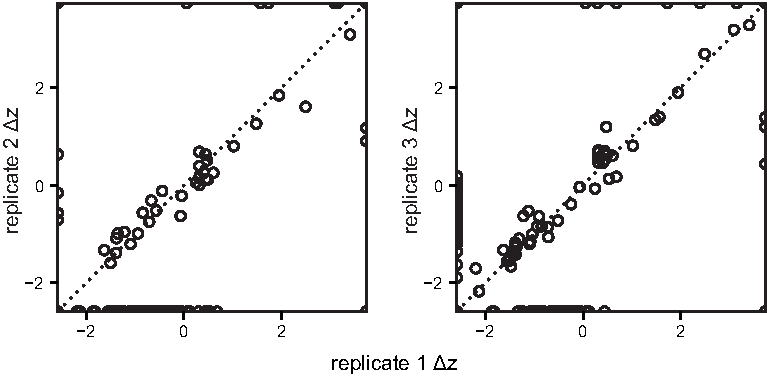
\includegraphics{texmex/fig/fig_3}
\caption*{{\bf Figure 3. OTUs in replicate units have correlated dynamics.}
The dynamics of OTUs (circles) in three replicate bioreactors (replicate 1,
$x$-axis; replicates 2 and 3, $y$-axes) inoculated with the same material and
subjected to the same conditions. The dotted line ($y=x$) indicates a perfect
correlation: an OTU on this line would have exactly the same $\Delta z$ in both
replicates, while deviations show differences in dynamics. For example, in the
left plot, OTUs above the dotted line experienced a greater increase in
abundance in replicate 2 than in replicate 1 (or, a smaller decrease in 2 than
in 1), while OTUs below the line ``grew more'' in replicate 2 than in replicate 1
(or, ``died less'' in 2 than in 1). OTUs with infinite $\Delta z$ are plotted on the
plot's borders (e.g., the points in the lower-right corner of the first plot
represent OTUs that have $\Delta z = +\infty$ in replicate 1 and $\Delta z = -\infty$ in replicate 2).}
\end{figure}

\clearpage
\begin{figure}
\centering
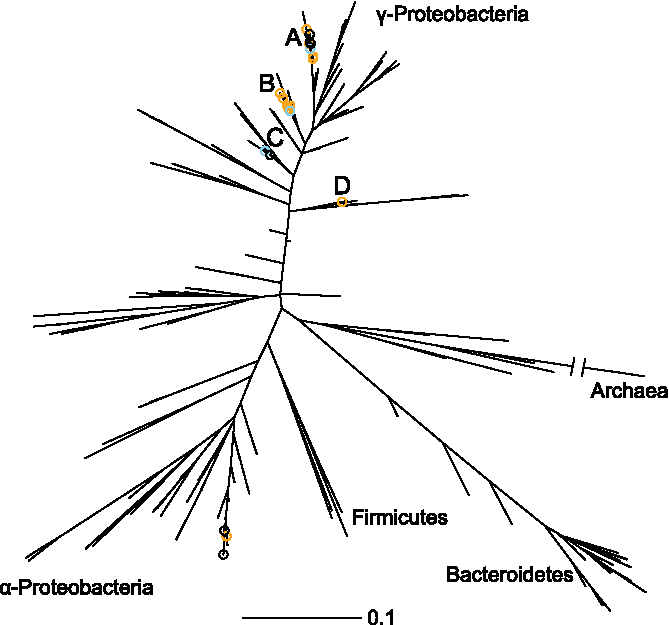
\includegraphics{texmex/fig/fig_4}
\caption*{{\bf Figure 4. OTUs that respond to oil appear in five clades.}
On a phylogenetic tree built from the 16S sequences, organisms potentially
responding to crude oil are marked with open circles. OTUs that satisfy the $\Delta z$
criteria are marked with blue circles, OTUs that satisfy the $\Delta F$ criteria are
marked with orange circles, and OTUs that satisfy both are marked with black
circles. Information about the taxonomy and dynamics of these sequences are
shown in Table 1. The five clades (A through E) are labeled, and select
taxonomic groups are labeled to help orient the reader. The Archaea branch is
truncated. Scale bar: substitutions per site.}
\end{figure}

\clearpage
\begin{table}
\caption*{{\bf Table 1. OTUs with dynamic behavior in response to amendment with oil}
(\textit{on next page}).
All OTUs that satisfied the $\Delta z$ or $\Delta F$ criteria are listed. The first
three columns show taxonomy. The most specific RDP taxonomic
classification with at least 80\% bootstrap support is shown. The next
two columns indicate whether the OTU satisfied the $\Delta z$ criteria, the $\Delta F$
criteria, or both. The next six columns show the changes in relative
abundance ($\Delta \mathrm{r.a.}$), rescaled reads $z$, and cumulative distribution
function $F$ in the control (``ct'') and experimental (``ex'') units. The
value $\Delta z = \mathrm{n.a.}$ is shown for OTUs that had zero counts at both
timepoints in that microcosm; $\Delta z = \infty$ is shown for OTUs had zero counts
before the treatment and more than zero counts after the treatment.}
\end{table}

\clearpage
\begin{landscape}
\begin{table}
\centering
\begin{tabular}{*{12}{l}}
\toprule
 &  &  & \multicolumn{2}{c}{criteria} & \multicolumn{2}{c}{$\Delta\mathrm{r.a.}$} & \multicolumn{2}{c}{$\Delta z$} & \multicolumn{2}{c}{$\Delta F$} &  \\
\cmidrule(r){4-5} \cmidrule(r){6-7} \cmidrule(r){8-9} \cmidrule(r){10-11}
Clade & Classification & support & $\Delta z$ & $\Delta F$ & ct & ex & ct & ex & ct & ex & OTU ID \\
\midrule
A & \textit{Maricurvus} & 0.95 & * &  & 0.033 & 0.739 & 1.382 & 1.419 & $-0.0002$ & 0.0041 & 3 \\
 & \textit{Maricurvus} & 0.87 &  & * & 0 & 0.008 & n.d. & $\infty$ & 0 & 0.9958 & 63 \\
 & $\gamma$-Proteobacteria & 1 &  & * & 0 & 0.0033 & n.d. & $\infty$ & 0 & 0.9942 & 107 \\
 & \textit{Maricurvus} & 0.87 &  & * & 0 & 0.003 & n.d. & $\infty$ & 0 & 0.9939 & 111 \\
 & \textit{Maricurvus} & 0.96 & * & * & 0 & 0.0013 & 0.827 & $\infty$ & 0.1429 & 0.9883 & 119 \\
 & \textit{Maricurvus} & 0.97 & * &  & $-0.0002$ & 0.0002 & 0.115 & $\infty$ & 0.0263 & 0.9292 & 256 \\
 & \textit{Maricurvus} & 0.9 & * &  & $-0.0001$ & 0.0005 & 0.402 & $\infty$ & 0.1649 & 0.9659 & 262 \\
 & \textit{Maricurvus} & 0.94 &  & * & 0 & 0.0007 & n.d. & $\infty$ & 0 & 0.9767 & 291 \\
B & \textit{Pseudomonas} & 1 & * &  & 0.0027 & 0.0629 & 1.137 & 1.073 & 0.014 & 0.0063 & 14 \\
 & \textit{Pseudomonas} & 0.99 &  & * & 0 & 0.0142 & n.d. & $\infty$ & 0 & 0.9961 & 42 \\
 & \textit{Pseudomonas} & 0.91 &  & * & 0 & 0.0112 & n.d. & $\infty$ & 0 & 0.996 & 53 \\
 & Pseudomonaceae & 0.82 &  & * & 0 & 0.0045 & n.d. & $\infty$ & 0 & 0.995 & 88 \\
 & \textit{Pseudomonas} & 0.99 &  & * & 0 & 0.0025 & n.d. & $\infty$ & 0 & 0.9931 & 120 \\
 & \textit{Pseudomonas} & 0.91 &  & * & 0 & 0.0018 & n.d. & $\infty$ & 0 & 0.9913 & 167 \\
 & \textit{Pseudomonas} & 1 &  & * & 0 & 0.0016 & n.d. & $\infty$ & 0 & 0.9903 & 174 \\
C & \textit{Alcanivorax} & 1 & * & * & $-0.0001$ & 0.0004 & 0.402 & $\infty$ & 0.1649 & 0.9599 & 206 \\
 & \textit{Alcanivorax} & 1 & * &  & $-0.0007$ & $-0.0001$ & 0.007 & $-0.143$ & $-0.0143$ & 0.0148 & 270 \\
D & \textit{Methylophaga} & 1 &  & * & 0 & 0.0006 & n.d. & $\infty$ & 0 & 0.9739 & 210 \\
E & Rhodobacteraceae & 1 & * & * & $-0.0003$ & 0.0008 & $-0.167$ & $\infty$ & $-0.1188$ & 0.9799 & 104 \\
 & Rhodobacteraceae & 1 & * & * & 0.0003 & 0.0003 & 1.237 & $\infty$ & 0.2935 & 0.9384 & 105 \\
 & Rhodobacteraceae & 1 & * & * & $-0.0002$ & 0.0001 & 0.115 & $\infty$ & 0.0263 & 0.7678 & 226 \\
 & Rhodobacteraceae & 1 &  & * & 0 & 0 & n.d. & $\infty$ & 0 & 0.6098 & 288 \\
\bottomrule
\end{tabular}
\end{table}
\end{landscape}

\clearpage
\begin{figure}[ht]
\centering
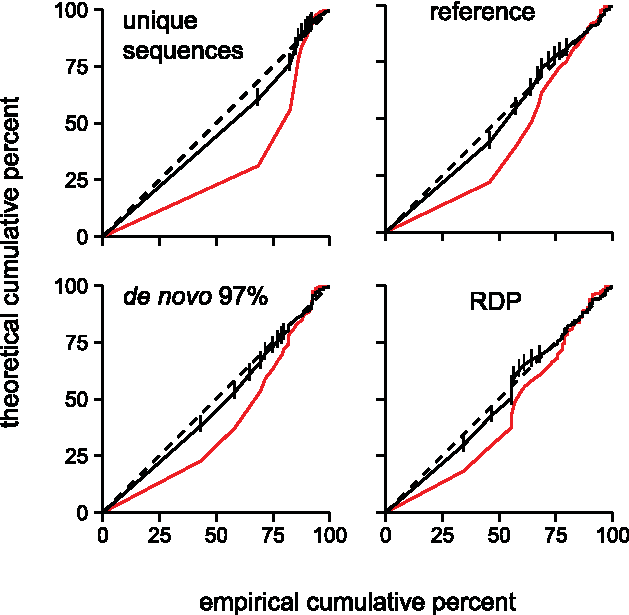
\includegraphics{texmex/fig/fig_s1}
\caption*{{\bf S1 Fig. TPL fits OTUs called by different methods.}
Probability-probability plots
comparing the empirical cumulative distribution function ($x$-axis) with the
theoretical cumulative probability of a TPL distribution fit to the
distribution of OTUs computed using different OTU-calling methods ($y$-axis,
black line). This is same ocean sample as in Figures 1 and 2. The first ten
data points are marked with vertical dashes: the first dash (furthest lower
left) represents fraction of OTUs with 1 read, the second dash represents the
fraction of OTUs with 2 or fewer reads, and so forth. The dotted black line
indicates a perfect fit ($y = x$). The theoretical cumulative probability of a
simple lognormal distribution fit to each OTU distribution (red) is shown to
emphasize the quality of the TPL fit. The methods are unique sequences (i.e.,
100\% identity OTUs; top left), 97\% reference-based OTUs from Greengenes (top
right), \textit{de novo} 97\% OTUs (bottom left), and genus-level OTUs computed with RDP
(bottom right). The empirical goodness-of-fit test described in the main text
yields $p = 0.35, 0.40, 0.44, 0.41$ for these data.}
\end{figure}

\clearpage
\begin{figure}[ht]
\centering
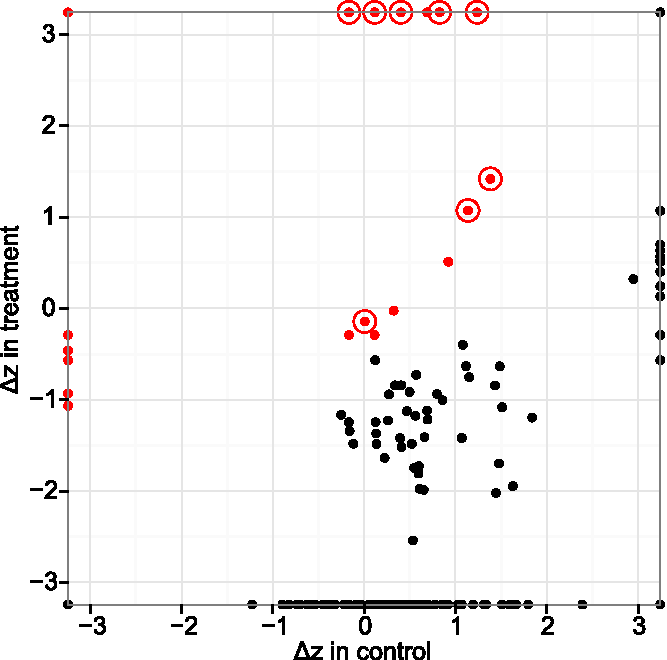
\includegraphics{texmex/fig/fig_s2}
\caption*{{\bf S2 Fig. OTU dynamics measured by $\Delta z$.}
Each OTU present in the microcosm experiment described in the main text is
shown. OTUs that meet the $\Delta z$ criterion described in the text ($\Delta z$ in treatment >
$\Delta z$ in control $- 0.5$) are in red. OTUs that meet the criterion and are among
the 304 most abundant sequences in the four microcosm experiments (i.e., those
shown as blue dots in Figure 4) are circled. OTUs with an undefined $\Delta z$ value in
either microcosm are not shown, while OTUs with infinite $\Delta z$ values are shown at
the border of the figure (e.g., an OTU with $\Delta z = +\infty$ in the control unit and $-\infty$
in the experimental unit would be shown in the lower-left corner).}
\end{figure}

\clearpage
\begin{figure}[ht]
\centering
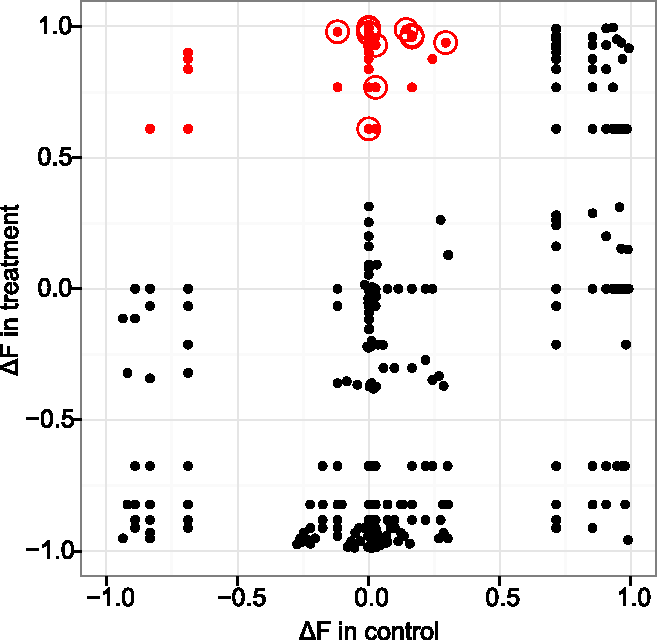
\includegraphics{texmex/fig/fig_s3}
\caption*{{\bf S3 Fig. OTU dynamics measured by $\Delta F$.}
Each OTU present in the microcosm experiment described in the main text is
shown. OTUs that meet the $\Delta F$ criteria described in the text ($\Delta F$ in treatment >
0.5; $\Delta F$ in control $< 0.5$) are in red. OTUs that meet those criteria and are
among the 304 most abundant sequences in the four microcosm experiments (i.e.,
those shown as red dots in Figure 4) are circled.}
\end{figure}
